
\section{ Extracting thermal impedances using FEA simulations}

The method used to extract thermal impedances for each module component, as well as common thermal
pathways in the petal, is the same as the one used for the barrel model. Several special simulation
runs are performed in which one component is powered on while the others are powered off. The results
are used to calculate all thermal resistances using the system of equations relating the resistances
to one another. (Note that this strategy is the same one as used in the barrel to extract thermal
impedances.)

If a component (e.g. the FEAST) is powered on the module, then the temperatures of each component
can be expressed as:
%
\begin{align}
\Delta T_\text{FEAST} =& P_\text{FEAST} \cdot (R_\text{FEAST} + R_{CM}) \label{eq:powered}\\
\Delta T_\text{ABC}   =& P_\text{FEAST} \cdot R_{CM}\\
\Delta T_\text{HCC}   =& P_\text{FEAST} \cdot R_{CM}\\
\Delta T_\text{AMAC}  =& P_\text{FEAST} \cdot R_{CM}\\
\Delta T_\text{Sensor}=& P_\text{FEAST} \cdot R_{CM}
\end{align}

By measuring\footnote{
``Measuring'' in this case means running the thermal FEA and extracting the temperatures of each
component.
} $\Delta T_{X}$ of all $X$ components when the FEAST is powered by a known amount, we can
extract $R_{CM}$ (which is overconstrained) and, inputting the measured $R_{CM}$ into the first
equation, we can then extract $R_\text{FEAST}$.

We can repeat the procedure by individual simulations where the HCCs only are powered, and when the
ABCs only are powered, to obtain 8 additional ``independent measurements'' of $R_{CM}$ and to
extract $R_\text{ABC}$ and $R_\text{HCC}$.

\subsection{Setup of the FEA Simulation to extract thermal impedances}

For a more complete description of the FEA model itself, including a complete description of the
thermal properties of the materials used to model the petal, see
\url{https://cds.cern.ch/record/2294921}.

For the special runs,
representative power numbers are used to power each component. In each simulation run, all instances
of one type of component (e.g. the ABCs) are powered on in all six modules, keeping the rest
off.\footnote{Powering all instances of one type of component is intended to capture effects of
cross-talk between modules.}
Average temperatures are measured for the HCC, ABC, FEAST, AMAC and sensor.

\def\thcc{\ensuremath{\overline{T}_\text{nHCC}}}
\def\tabc{\ensuremath{\overline{T}_\text{nABC}}}
\def\tfeast{\ensuremath{\overline{T}_\text{FEAST}}}
\def\tsensor{\ensuremath{T_\text{sensor}}}
\def\Rm{\ensuremath{{\text{R}m}}}

A brief description of each component and its properties, as well as other details
of the simulation, is below:
\begin{itemize}
\item FEAST: the current FEA models the feast as a $3\times3$~mm$^2$ $\times~350~\mu$m chip inside
the shield box. The actual FEAST should be a $3\times3$~mm$^2$ chip on top of a $3.6\times3.6$~mm$^2$
copper pad. Thus, the thermal impedances obtained here should be conservative. We will 
consider scaling the thermal impedance down by a factor of ($3.6\times3.6$)/($3\times3$).
\item AMAC: a $3\times3$~mm $\times~350~\mu$m chip, roughly in the center of the power board.
  \begin{itemize}
    \item The AMAC is powered using regulators located in the FEAST chip, with a power dissipation
      of the regulators corresponding to the voltage drop in the regulator (0.415~W) -- see Eq.~\ref{eq:amac_regulator}.
  \end{itemize}
\item EOS: The placement of the EOS power sources is not exact, but this should have a small impact
  on the results.
\item Cooling: The heat transfer coefficient used in simulation is a constant 8000~W/m$^{2}$K.
  The coolant temperature is set at $-30$~C; convection is not modeled.
\end{itemize}




\subsection{FEA Simulation Runs to extract thermal impedances}

For the extraction of the thermal impedances, a simplified set of input power parameters are used,
summarized in Table~\ref{tab:simulation_runs}.
In the FEA, the power is distributed over all 6 surfaces (which is understood to be different from
the barrel treatment of this study).

\let\arraystretcha\arraystretch
\renewcommand\arraystretch{1.4} % 1.6
\begin{table}[h!]
\begin{center}
\adjustbox{max width=\textwidth}{ %% just before tabular
\begin{tabular}{|l|l|l|l|} \hline
Simulation \# & Description                        & Input parameters           \\ \hline
[0]           & The nominal petal simulation       & Nominal -- not used to extract impedances \\
1             & All HCCs powered on, rest off      & $P_\text{HCC}=0.413$~W     \\
2             & All ABCs powered on, rest off      & $P_\text{ABC}=0.149$~W     \\
3             & All FEASTs powered on, rest off    & $P_\text{FEAST}=1.5$~W$^*$ \\
%% \hline
%% \multicolumn{3}{|c|}{Extended simulations} \\ \hline
%% 4             & Tape ``powered'' on, rest off      & skip for now \\
%% 5             & HVMUX powered on, rest off         & skip for now \\
%% 6             & R$_\text{HV}$ powered on, rest off & skip for now \\
%% 7             & EOS                                & skip for now \\ % $P_\text{EOS}=3.03$~W$^{**}$
\hline \end{tabular}
} %% resizebox after tabular
\end{center}
\caption{ Description of the 3 thermal simulations required to obtain the thermal impedances.
}
\label{tab:simulation_runs}
\end{table}
\let\arraystretch\arraystretcha

$^*$ The actual nominal power of the FEAST varies for each module; however, for the simulation to extract
the thermal impedances, the power is set to 1.5~W for all FEASTs in the petal.\\
%
Note also that in R3, the 1.5~W are shared by two FEASTs, each with 0.75~W of power.




\subsection{Measurements performed in each FEA Special Simulation}

%% For each component, the temperature measured is the average of the top surface nodes of all
%% components of a given type, in a given module.

The average, min and max temperatures are taken over the volume of the elements.
%
The average/min/max temperatures for a given component are taken as the average/min/max of the
component on either side of the petal (e.g. the R0 FEAST average temperature is taken as the average of
the R0 FEASTs on the front and back sides).

\begin{itemize}
\item $(\thcc)_\Rm$: The average HCC temperature of the $n$ HCCs in the module, for each module R$m$ (R0, R1, ... R5) (6~total)
\item $(\tabc)_\Rm$: The average ABC temperature of the $n$ ABCs in the module, for each module R$m$ (6~total)
\item $(\tfeast)_\Rm$: The temperature of the FEAST in the module, for each module R$n$ (6~total)
\item \tsensor, taken for R0, R1, R2, R3, R4, R5 (6~total)
\begin{itemize}
  \item $\tsensor^\text{Avg}$: The average sensor temperature taken over the volume of the sensor
  \item $\tsensor^\text{Max}$: The maximum sensor temperature in the module, for each module
  \item $\tsensor^\text{Min}$: The minimum sensor temperature in the module, for each module
\end{itemize}
\item $T_\text{EOS}$, to obtain the thermal impedance of the thermal pathway of the EOS.
\end{itemize}

Figure~\ref{thermal_data} shows the raw data of the special run simulations. 

\begin{figure}[ht!]
\begin{subfigure}[t]{0.50\textwidth}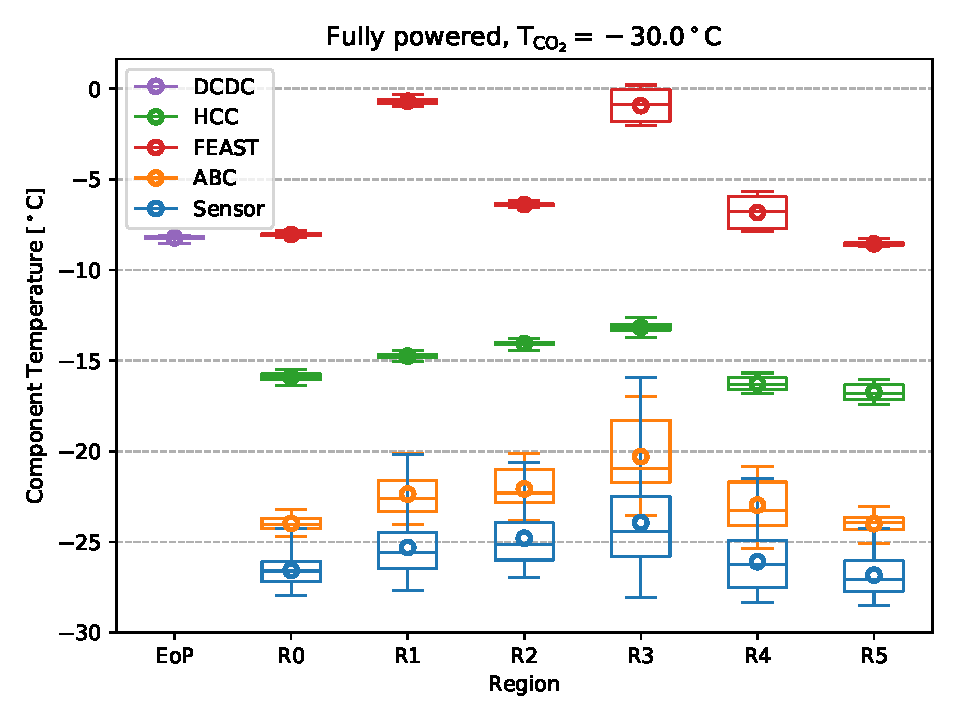
\includegraphics[width=0.99\linewidth]{figures/FEA_20171207_m30p0C_0p0Wm2C_DP1_ALL_S0.pdf}\vspace{-3mm}\caption{Simulation 0}\end{subfigure}
\begin{subfigure}[t]{0.50\textwidth}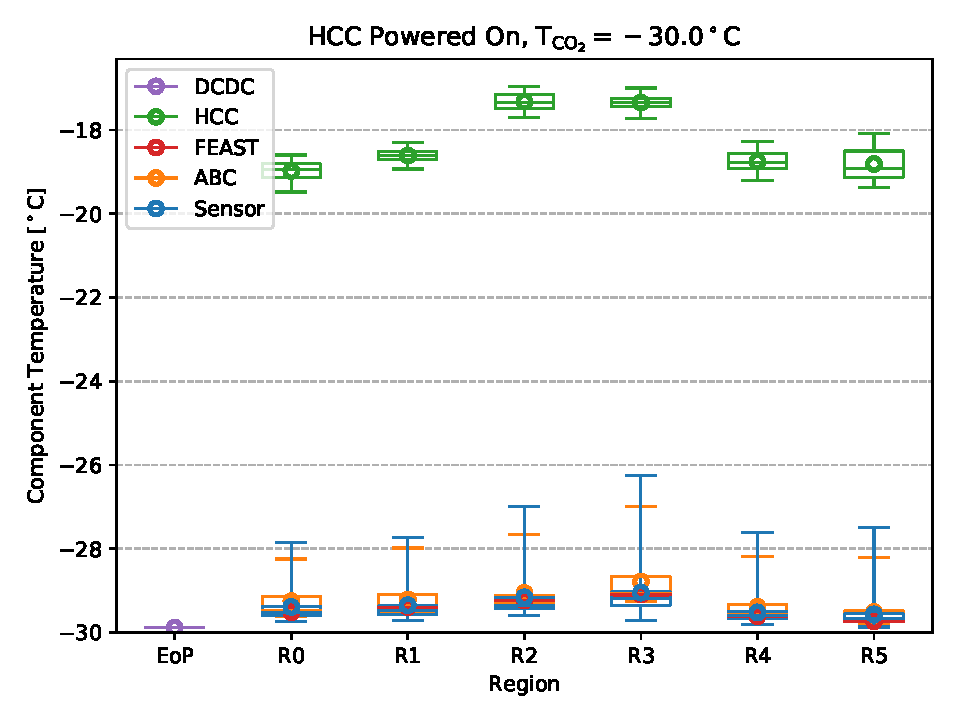
\includegraphics[width=0.99\linewidth]{figures/FEA_20171207_m30p0C_0p0Wm2C_DP1_ALL_S1.pdf}\vspace{-3mm}\caption{Simulation 1}\end{subfigure}\vspace{5mm}\\ 
\begin{subfigure}[t]{0.50\textwidth}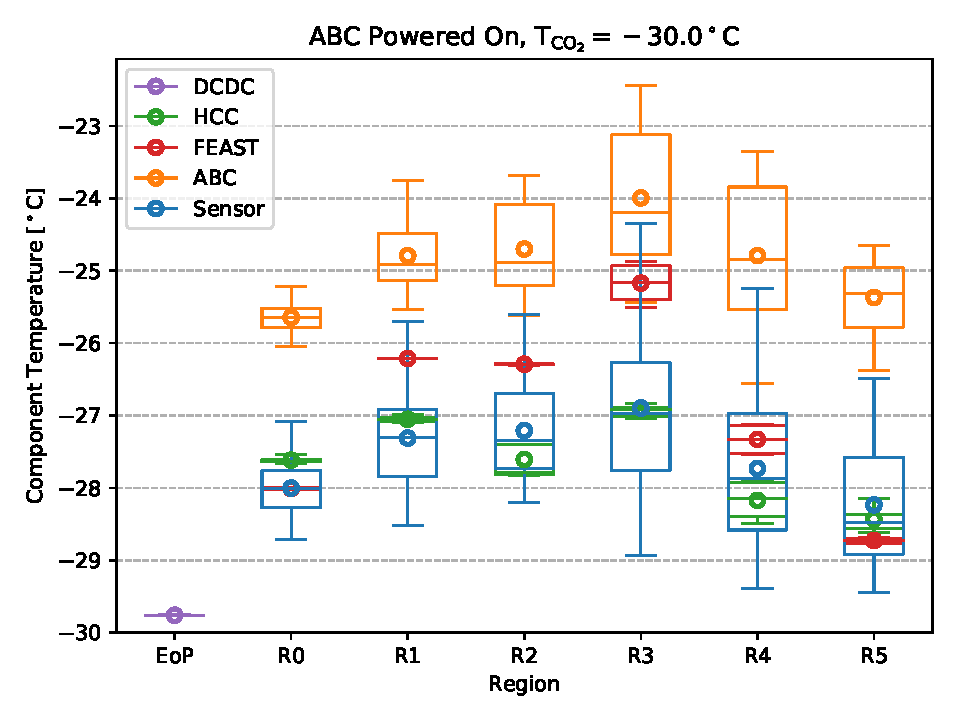
\includegraphics[width=0.99\linewidth]{figures/FEA_20171207_m30p0C_0p0Wm2C_DP1_ALL_S2.pdf}\vspace{-3mm}\caption{Simulation 2}\end{subfigure}
\begin{subfigure}[t]{0.50\textwidth}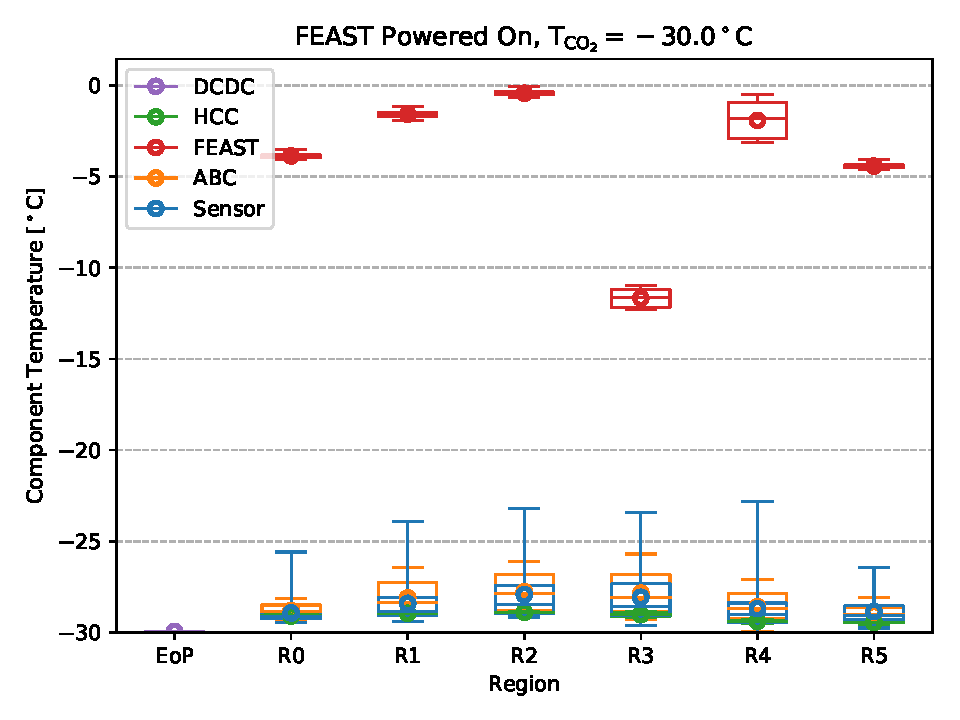
\includegraphics[width=0.99\linewidth]{figures/FEA_20171207_m30p0C_0p0Wm2C_DP1_ALL_S3.pdf}\vspace{-3mm}\caption{Simulation 3}\end{subfigure}
\caption{Box-and-whisker plot of the four simulation scenarios described in Table~\ref{tab:simulation_runs}.
The box is the interquartile range (middle 50\%) of the component's temperature, and the whiskers are
the minimum and maximum temperatures.}
\label{thermal_data}
\end{figure}

\clearpage

\subsection{Thermal impedance results from the FEA data}

Figure~\ref{rcm_fits} presents the data from the special FEA runs used to calculate $R_{CM}$ in each
module; this value is extracted by fitting the data points using the equation
$\Delta T= P\cdot R_{CM}$. A few points are excluded from the fit to data because of either too-remote
or too-close
proximity between the powered component and the component whose temperature is measured. 
This applies to the AMAC and FEAST in R4 and R5 when the HCC is powered--the HCC is fairly thermally 
isolated from these two components. In R0, the opposite effect occurs: the AMAC and FEAST are too
close and share a common thermal pathway, so the AMAC measurement is ignored when the FEAST is powered.
Except for these cases, all other data points are used to fit for $R_{CM}$.

\begin{figure}[ht!]
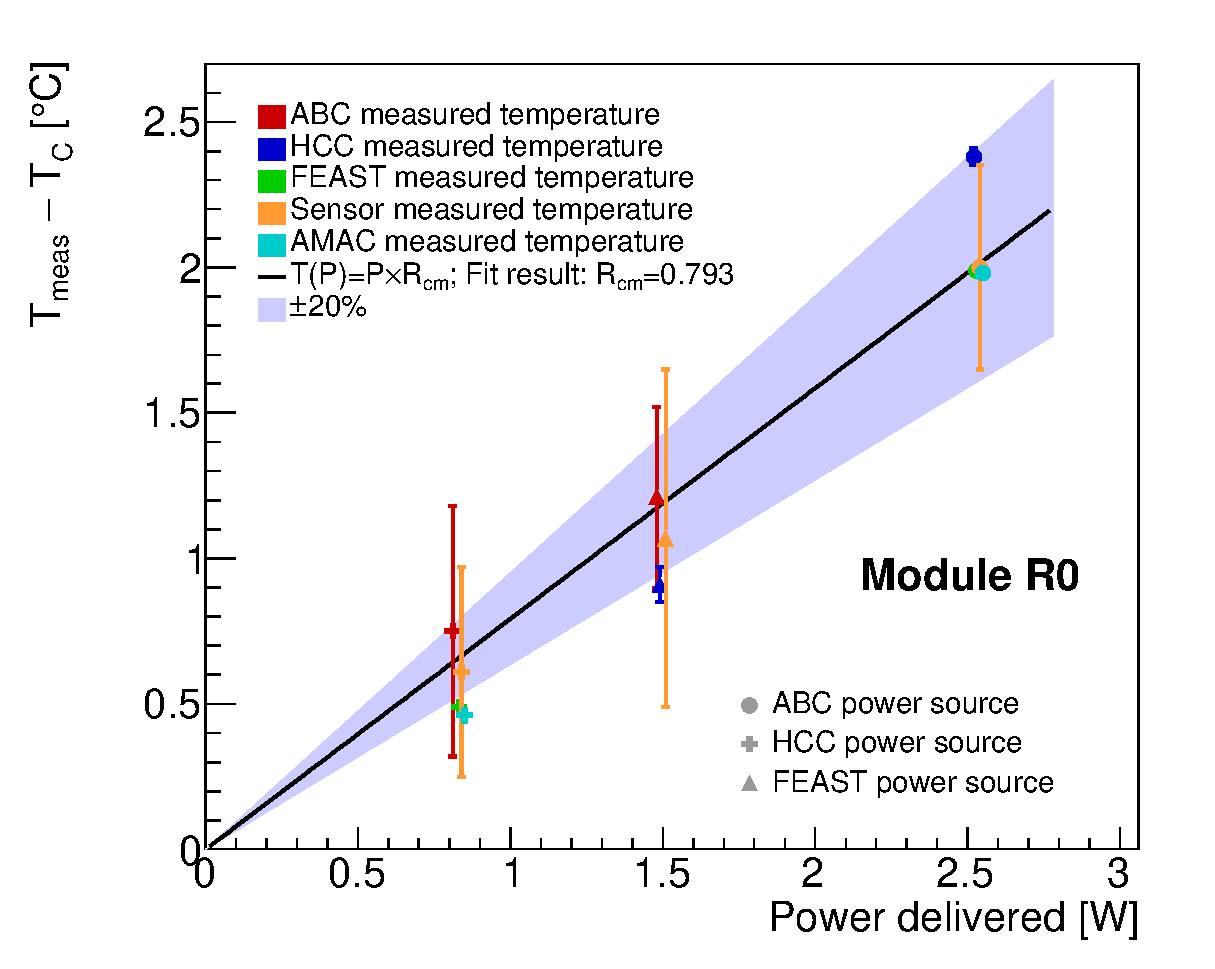
\includegraphics[width=0.49\linewidth]{figures/ThermalImpedanceFit_R0_Rcm.eps}
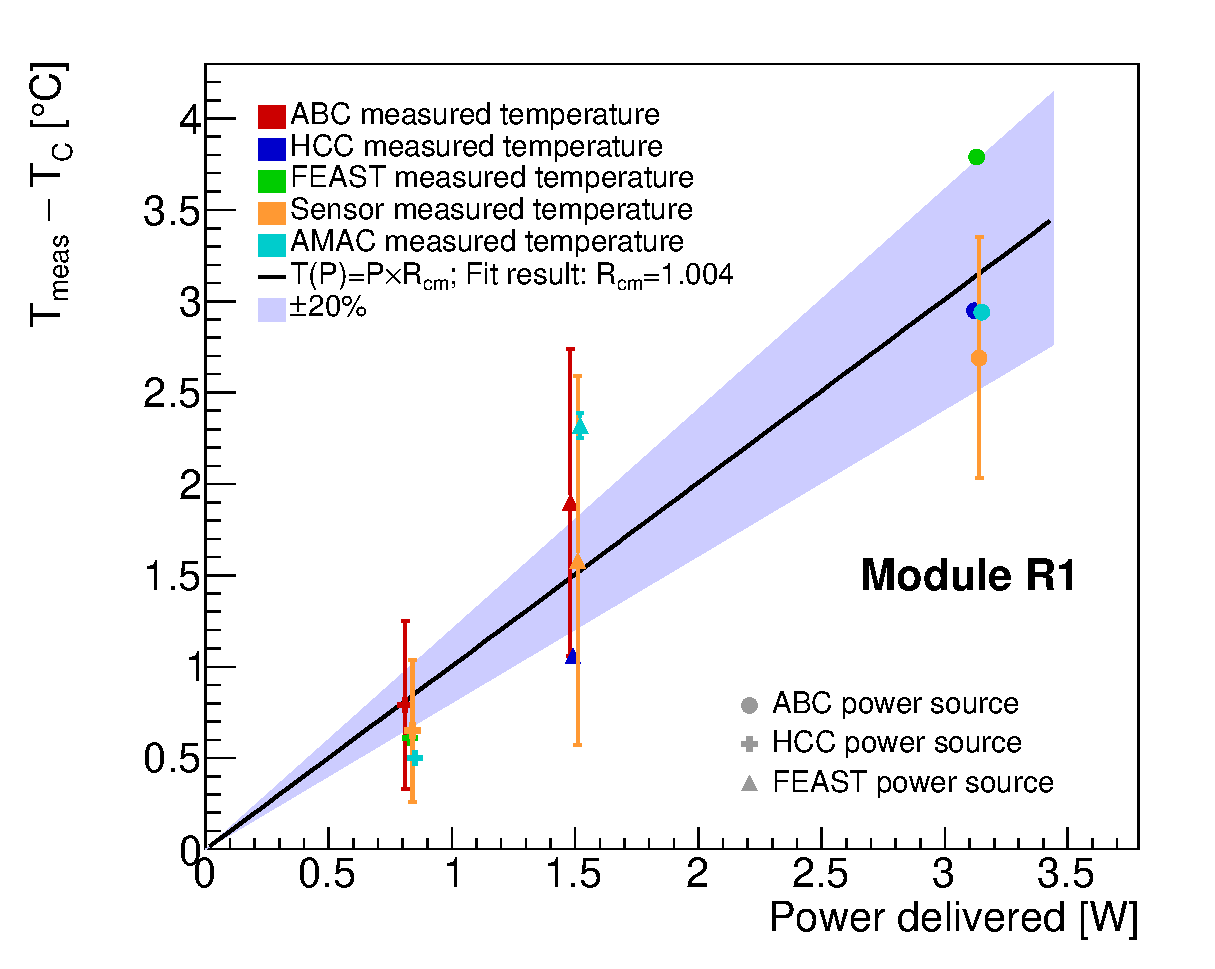
\includegraphics[width=0.49\linewidth]{figures/ThermalImpedanceFit_R1_Rcm.eps}\\
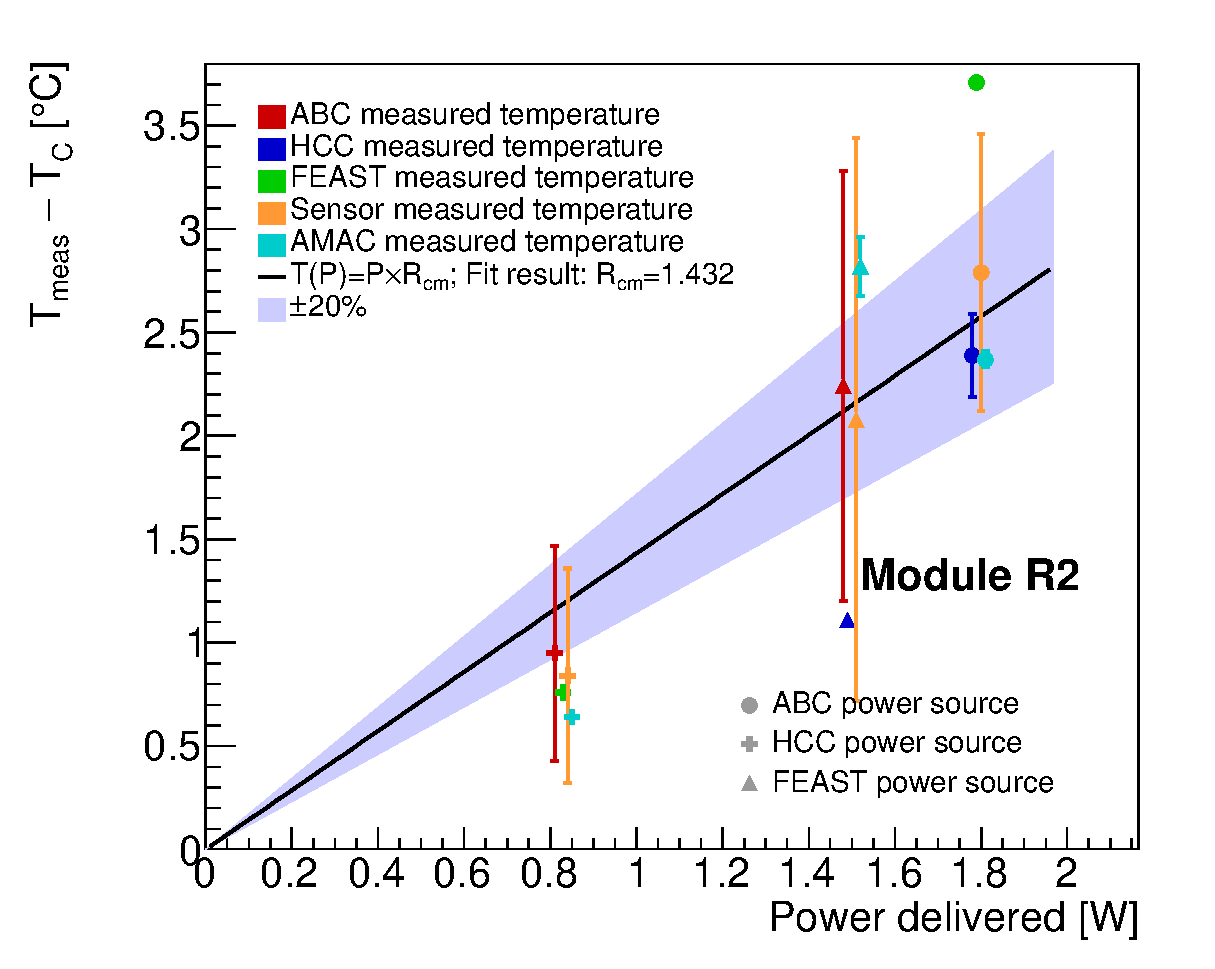
\includegraphics[width=0.49\linewidth]{figures/ThermalImpedanceFit_R2_Rcm.eps}
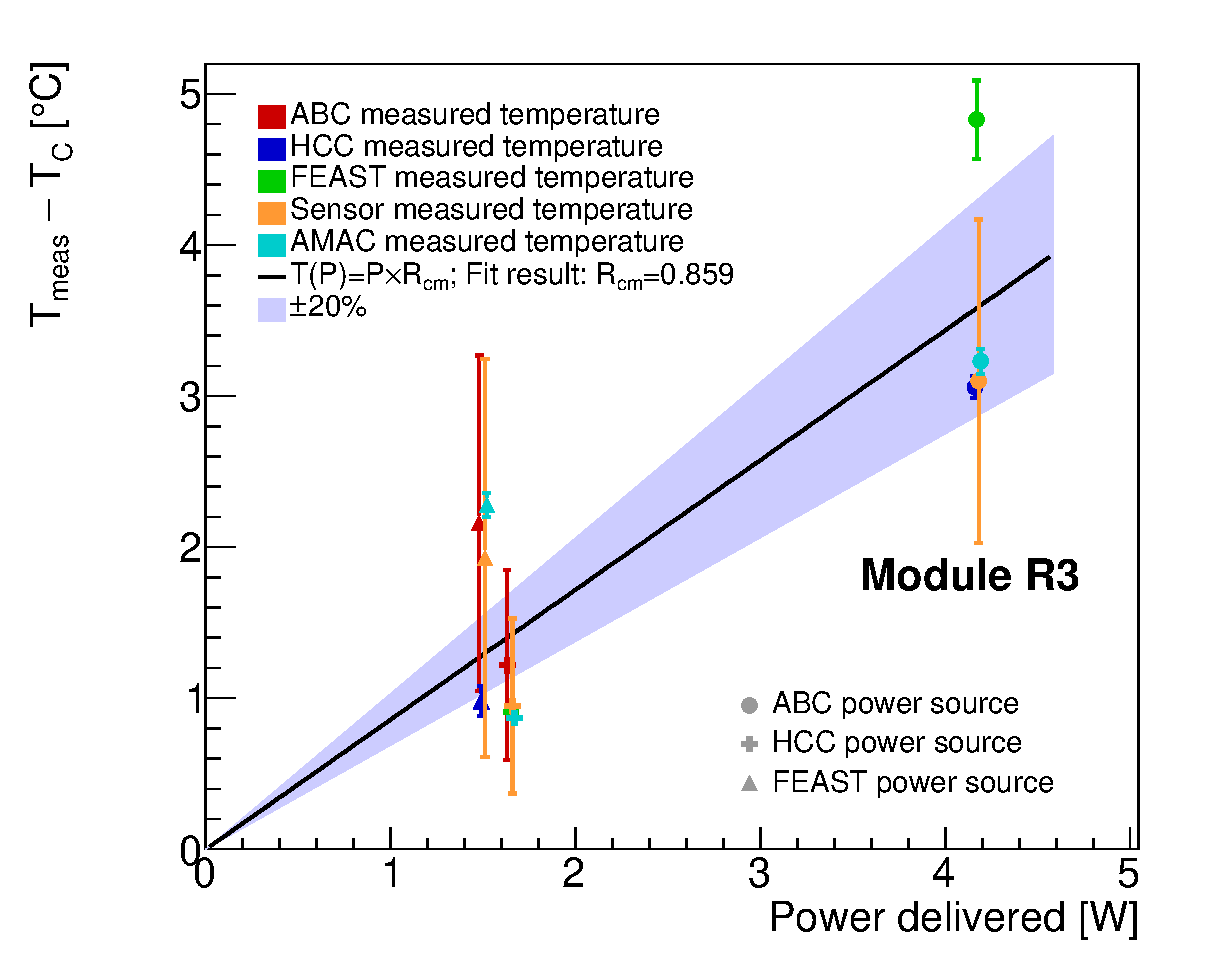
\includegraphics[width=0.49\linewidth]{figures/ThermalImpedanceFit_R3_Rcm.eps}\\
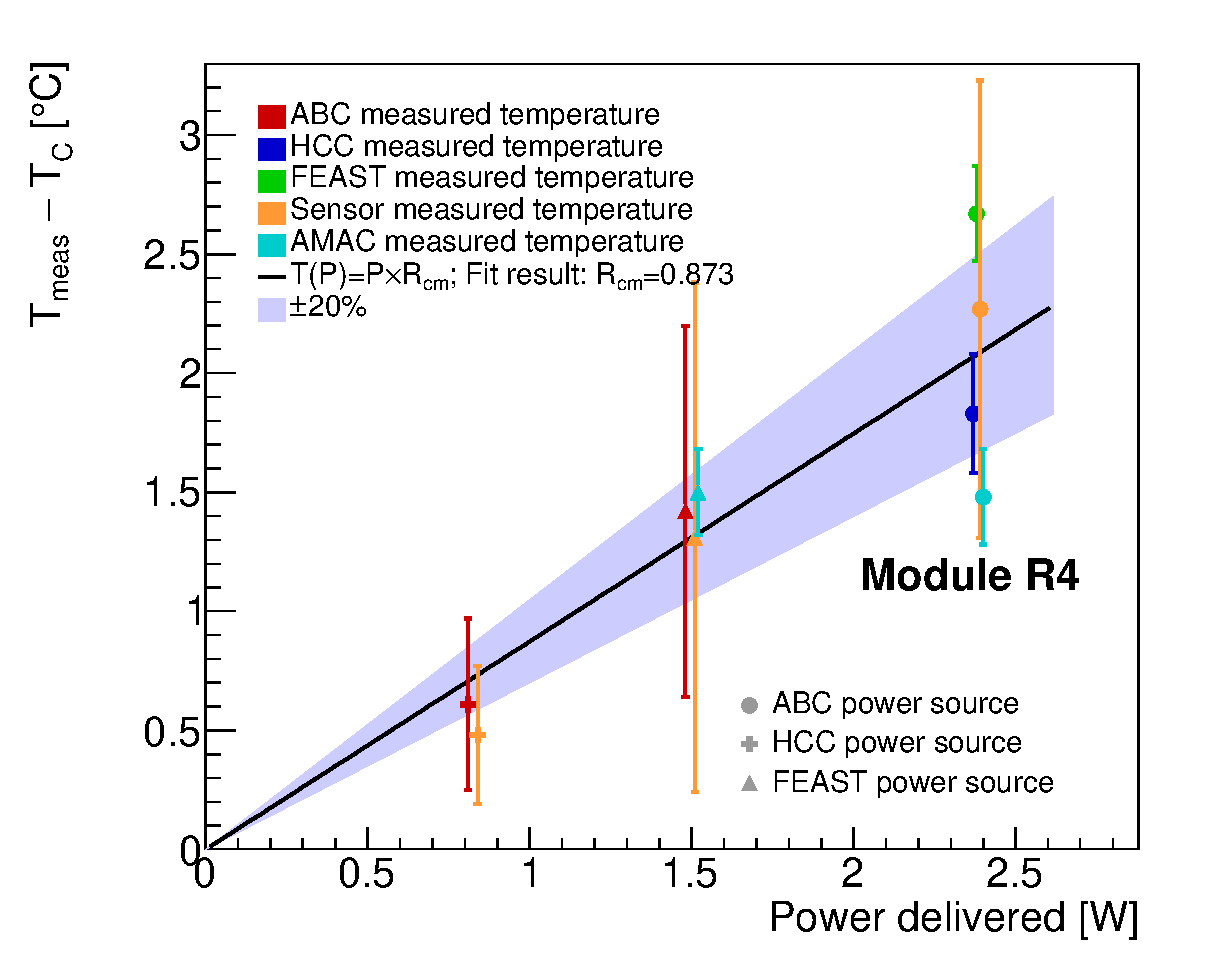
\includegraphics[width=0.49\linewidth]{figures/ThermalImpedanceFit_R4_Rcm.eps}
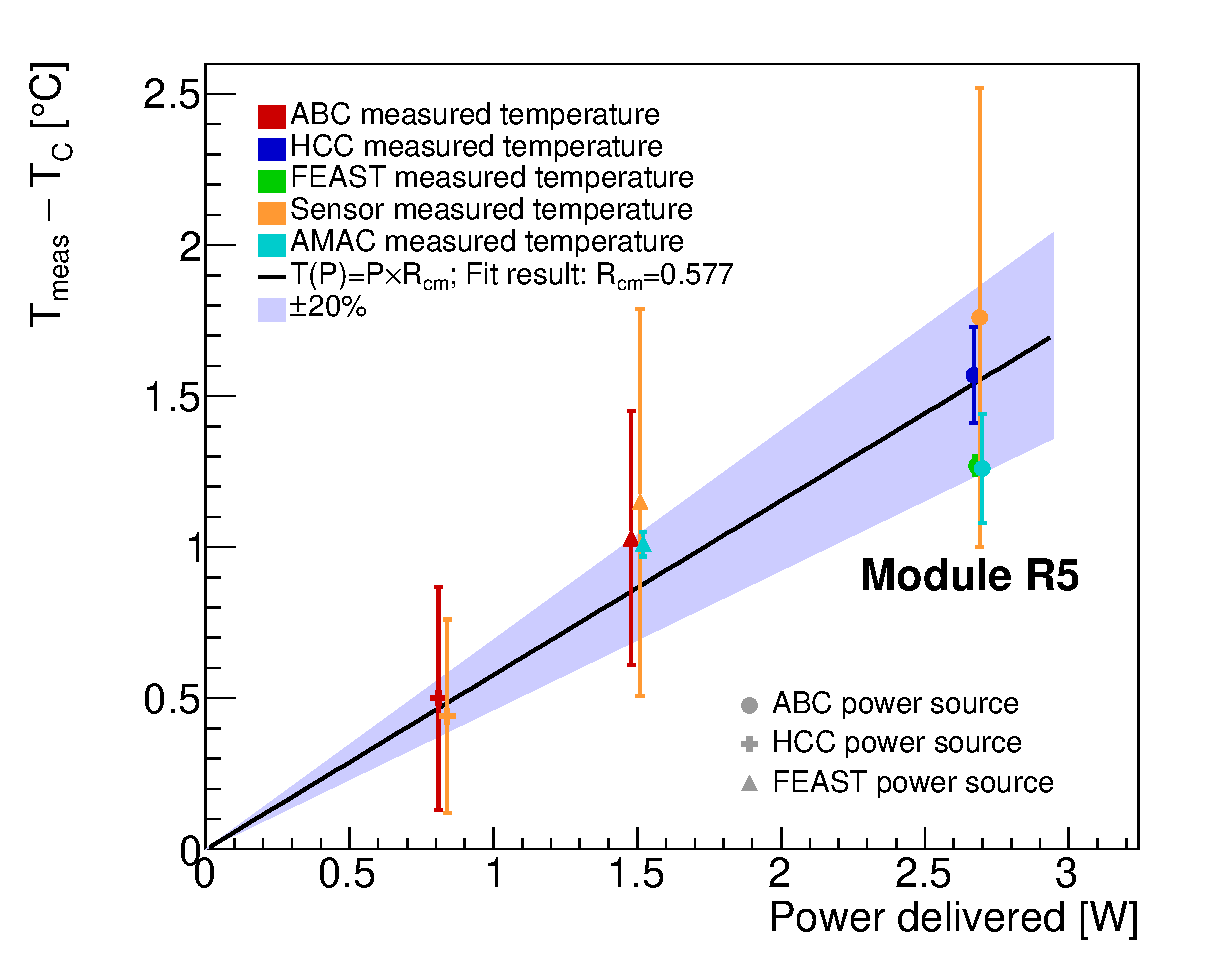
\includegraphics[width=0.49\linewidth]{figures/ThermalImpedanceFit_R5_Rcm.eps}
\caption{Measurements of $\Delta T$ of module components when certain components (ABC, HCC, FEAST)
are powered on with the values given in Table~\ref{tab:simulation_runs}. 
The error bars represent the standard deviation of temperatures of that particular
component. A fit to the slope of the data determines $R_{CM}$; note that the fit does not consider
the error bars shown, i.e. in the fit all errors are 0.
}
\label{rcm_fits}
\end{figure}

Once $R_{CM}$ is determined, it can be plugged into equations like Eq.~\ref{eq:powered} to extract
$R_\text{FEAST}$, $R_\text{ABC}$ and $R_\text{HCC}$.
Table~\ref{tab:thermal_impedances} shows the thermal impedances calculated
from the FEA simulations.

%% \def\insulabc{$R_\text{ABC}\times n_\text{ABC}$\xspace}
%% \def\insulhcc{$R_\text{HCC}\times n_\text{HCC}$\xspace}
\def\insulabc{$(R\times n)_\text{ABC}$\xspace}
\def\insulhcc{$(R\times n)_\text{HCC}$\xspace}
\def\insulfeast{$(R\times n)_\text{FEAST}$\xspace}

%
\let\arraystretcha\arraystretch
\renewcommand\arraystretch{1.1} % 1.6
\begin{table}[h]
\begin{center}
\adjustbox{max width=\textwidth}{ %% just before tabular
\begin{tabular}{|l|cc|c|c|c|c|c|c|} \hline
       &             &              &  \multicolumn{2}{c|}{FEAST}     & \multicolumn{2}{c|}{ABC}   & \multicolumn{2}{c|}{HCC}   \\
Module & $R_C$ [K/W] & $R_M$ [K/W]  & $ R_\text{FEAST}$ & \insulfeast & $R_\text{ABC}$ & \insulabc & $R_\text{HCC}$ & \insulhcc \\ \hline
R0     & \multicolumn{2}{c|}{0.793} &            16.627 &      16.627 &          0.927 &    15.759 &         12.485 &    24.970 \\
R1     & \multicolumn{2}{c|}{1.004} &            17.936 &      17.936 &          0.661 &    13.881 &         12.719 &    25.438 \\
R2     & \multicolumn{2}{c|}{1.432} &            18.282 &      18.282 &          1.529 &    18.348 &         13.833 &    27.666 \\
R3     & \multicolumn{2}{c|}{0.859} &            11.361 &      22.722 &          0.582 &    16.296 &\phantom{0}6.808&    27.232 \\
R4     & \multicolumn{2}{c|}{0.826} &            17.847 &      17.847 &          1.316 &    21.056 &         12.669 &    25.338 \\
R5     &              0.091 & 0.486 &            16.470 &      16.470 &          1.151 &    20.718 &         12.905 &    25.810 \\ \hline
SS EOS    &           0.719 & 0.393      & \multicolumn{2}{c|}{19.650} &         1.003 &    20.060 &         12.305 &    24.610 \\
SS middle &   \multicolumn{2}{c|}{1.160} & \multicolumn{2}{c|}{19.752} &         0.928 &    18.560 &         13.157 &    26.314 \\
LS EOS    &           0.811 & 0.427      & \multicolumn{2}{c|}{19.602} &         2.194 &    21.940 &         24.195 &    24.195 \\
LS middle &   \multicolumn{2}{c|}{1.360} & \multicolumn{2}{c|}{19.663} &         2.141 &    21.410 &         25.174 &    25.174 \\
%% in [degC/W]  RC       RM       RS      REOS    RABC     RHCC      RFEAST
%% SS EOS       0.719    0.393    0.02    15.0    1.003    12.305    19.650
%% SS middle    1.160             0.02       -    0.928    13.157    19.752
%% LS EOS       0.811    0.427    0.02    15.0    2.194    24.195    19.602
%% LS middle    1.360             0.02       -    2.141    25.174    19.663
\hline \end{tabular}
} %% resizebox after tabular
\end{center}
\caption{Effective thermal impedances calculated from Yu-Heng's numbers (in K/W).
For instances where you have $n$ components, the thermal insulance (inverse of HTC) is also calucated, simply
in units of {${(\text{Area}_\text{1-device})\cdot\text{K/W}}$}.
The short-strip (SS) and long-strip (LS) thermal impedances from the analogous barrel study are shown
for comparison (the ``$(R\times n)_X$'' values are comparable).
}
\label{tab:thermal_impedances}
\end{table}
\let\arraystretch\arraystretcha

\subsection{Other assumed thermal quantities}

Some thermal impedances are estimated roughly rather than calculated using detailed simulations.
These include:
%
\begin{itemize}
\item $R_\text{EOS}=15.0$~K/W (guessed by Georg/Graham)
\item $R_\text{sensor}=0.02$~K/W (guessed by Georg/Graham)
\item $R_\text{tape}=0.01$~K/W per module (i.e. there are 6 such resistors in the petal, one
for each module). This is considered a worst-case value.
\end{itemize}
%
The impact of an incorrect assumption on the above quantities is expected to be small.
